\documentclass[18pt]{beamer}
\usetheme{Madrid}

\usepackage{graphics}

\begin{document}

\title[Open Source]{Open Source Software Practices}
\subtitle[UH]{University of Houston}
\author[Luis Ibanez]{Luis Ibanez}
\institute{KITWARE Inc.\\
Clifton Park, NY
}
\date[April 2011]{April 6 2011}

\begin{frame}
\titlepage
\end{frame}

\begin{frame}
  \tableofcontents
\end{frame}


\section{Economics}

{
\setbeamertemplate{navigation symbols}{}  % optionally hide navigation buttons
\begin{frame}[plain]
\fontsize{72pt}{90pt}\selectfont
\center
\begin{center}
Economics
\end{center}
\end{frame}
}

\begin{frame}[plain]
\fontsize{36pt}{36pt}\selectfont
\center
\begin{center}
The Software\\
Manufacturing\\
Delusion
\end{center}
\end{frame}

\begin{frame}[plain]
\fontsize{18pt}{18pt}\selectfont
\center
\begin{quote}
Software is largely a \textbf{service} industry\\
operating under the persistent\\
but unfounded \textbf{delusion}\\
that it is a \textbf{manufacturing} industry.\\
\end{quote}
\bigskip
\begin{flushright}
Eric S. Raymond
\end{flushright}
\end{frame}


\begin{frame}[plain]
\frametitle{Sale Value versus Use Value}
  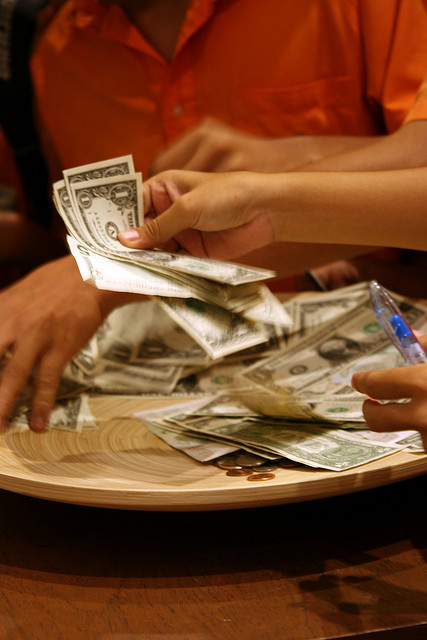
\includegraphics[width=0.5\textwidth,height=\paperheight]{../Art/2672465894_5b21e12135_z.jpg}
  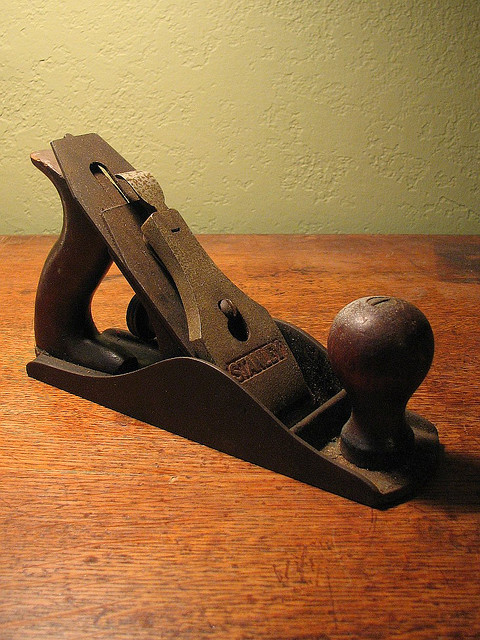
\includegraphics[width=0.5\textwidth,height=\paperheight]{../Art/4293485922_7474ef04ce_z.jpg}
\end{frame}


\begin{frame}
\frametitle{Some Notable Companies}

\begin{tabular}{lrrr}
\hline
\textbf{Publisher} &	\textbf{Annual Revenue} & \textbf{Cost of Revenue} & \textbf{Gross Profit} \\
\hline
\hline
\href{http://www.google.com/finance?fstype=ii\&q=NASDAQ:MSFT}{Microsoft Corp.}	& \$ 62,484 M & \$ 12,395 M  & \$ 50,089 M  \\
\hline
\href{http://www.google.com/finance?q=NYSE:IBM\&fstype=ii}{IBM Corp.} & \$ 95,759 M & \$ 51,972 M & \$ 43,787 M \\
\hline
\href{http://www.google.com/finance?q=NASDAQ:AAPL\&fstype=ii}{Apple Inc.} & \$ 42,905 M & \$ 25,683 M & \$ 17,222 M \\
\hline
\href{http://www.google.com/finance?q=NASDAQ:ORCL\&fstype=ii}{Oracle} & \$ 26,820 M & \$ 5,764 M & \$ 21,056 M \\
\hline
\href{http://www.google.com/finance?q=NASDAQ:SYMC\&fstype=ii}{Symantec}	&	\$ 5,985 M & \$ 1,105 M & \$ 4,880 M \\
\hline
\href{http://www.google.com/finance?q=NASDAQ:ADBE\&fstype=ii}{Adobe} & \$ 943 M & \$ 107 M & \$ 835 M \\
\hline
\end{tabular}

\bigskip
\begin{center}
Balance Sheets - September 2009 - September 2010
\end{center}

\end{frame}


\begin{frame}
\frametitle{Largest Software Vendors - 2010}

\begin{center}
\begin{tabular}{clrrr}
\hline
  \textbf{Rank} &\textbf{Vendor} &	\textbf{Software \$M} & \textbf{Total \$M} & \textbf{Percent} \\
\hline
\hline
1 &  \textbf{Microsoft} & 49,090  & 61,159 &  80\% \\
2 &  \textbf{IBM} & 21,396  & 95,758  & 22\% \\
3 &  \textbf{Oracle} & 18,582  & 22,734 &  82\% \\
4 &  SAP & 11,368  & 15,373 &  74\% \\
5 &  Ericsson & 7,595  & 29,014 &  26\% \\
6 &  Nintendo & 6,799  &  17,762 &  38\% \\
7 &  HP & 6,183  &  116,245 &  5\% \\
8 &  \textbf{Symantec} & 5,565  & 5,992 &  93\% \\
9 &  Nokia Siemens & 4,529  &  18,114 &  25\% \\
10&  Blizzard & 4,279  & 4,279 & 100\% \\
\end{tabular}

\vskip15pt
\scriptsize
\url{http://www.softwaretop100.org/global-software-top-100-edition-2010}\\

\end{center}
\end{frame}


\begin{frame}
\frametitle{Largest Software Vendors - 2010}

\begin{center}
\begin{tabular}{clrrr}
\hline
\textbf{Rank} &\textbf{Vendor} &	\textbf{Software \$M} & \textbf{Total \$M} & \textbf{Percent} \\
\hline
\hline
11 & CA & 4,012  & 4,318 & 93\% \\
12 & EMC & 3,960  & 14,026 & 28\% \\
13 & \textbf{Electronic Arts} & 3,728  &  3,728 & 100\% \\
14 & \textbf{Adobe} & 2,796 &  2,987 & 94\% \\
15 & Cisco & 2,137 & 36,633 & 6\% \\
16 & SunGard & 1,996  & 5,508 & 36\% \\
17 & Sony & 1,914 &  79,441 & 2\% \\
18 & BMC & 1,758& 1,888 & 93\% \\
19 & Alcatel-Lucent & 1,635  &  21,835 & 8\% \\
20 & Konami & 1,594 &  2,887 & 55\% \\
\end{tabular}

\vskip15pt
\scriptsize
\url{http://www.softwaretop100.org/global-software-top-100-edition-2010}

\end{center}
\end{frame}


\begin{frame}
\frametitle{Largest Software Vendors - 2010}

\begin{center}
\begin{tabular}{clrrr}
\hline
\textbf{Rank} &\textbf{Vendor} &	\textbf{Software \$M} & \textbf{Total \$M} & \textbf{Percent} \\
\hline
\hline
21 & Hitachi & 1,589 & 99,818 & 2\% \\
22 & Dassault & 1,584 & 1,803 & 88\% \\
23 & Infor & 1,575 & 2,100 & 75\% \\
24 & Sage & 1,557 & 2,336 & 67\% \\
25 & \textbf{Autodesk} & 1,557 & 1,764 & 88\% \\
\ldots & \ldots & \ldots & \ldots & \ldots \\
28 & \textbf{Apple} & 1,218 &	43,086 & 	\textbf{3\%}  \\
32 & SAS Institute & 1,155 	& 	2,310 &	50\%  \\
37 & VMWare & 1,029 &	2,024 & 	51\%  \\
39 & McAfee & 964 &	1,927 & 50\% \\
\end{tabular}

\vskip15pt
\scriptsize
\url{http://www.softwaretop100.org/global-software-top-100-edition-2010}

\end{center}
\end{frame}


{
\setbeamertemplate{navigation symbols}{}  % optionally hide navigation buttons
\begin{frame}[plain]
\fontsize{72pt}{90pt}\selectfont
\center
\begin{center}
\$ 13 Trillion
\end{center}
\end{frame}
}

{
\setbeamertemplate{navigation symbols}{}  % optionally hide navigation buttons
\begin{frame}[plain]
\fontsize{72pt}{90pt}\selectfont
\center
\begin{center}
\$ 13 Trillion
\end{center}
\end{frame}
}

{ % brace to limit the scope of \setbeamertemplate
\setbeamertemplate{navigation symbols}{}  % optionally hide navigation buttons
\setbeamertemplate{background canvas}{
  
\includegraphics[width=\paperwidth,height=\paperheight]{../Art/osi_symbol.png}
}
\begin{frame}[plain]
\end{frame}
} % closing brace

\section{Practices}

\begin{frame}
\frametitle{Governance}
\begin{itemize}
\item Benevolent Dictator
\pause
\item Bazaar
\end{itemize}
\end{frame}


\begin{frame}
\frametitle{Credits}
\begin{itemize}
\item \url{http://opensource.org/files/osi_standard_logo.png}
\item \url{http://www.flickr.com/photos/lifeontheedge/2672465894}
\item \url{http://www.flickr.com/photos/hortulus_aptus/4293485922}
\end{itemize}
\end{frame}

\end{document}
